%: O
%: TD shapes and sketches...

\ifx\wholebook\relax\else
\input{../Common.tex}
\input{../macroes.tex}
\begin{document}
\fi


\chapter{Fun with Robots}\label{cha:custo}

\begin{chapterfigure}
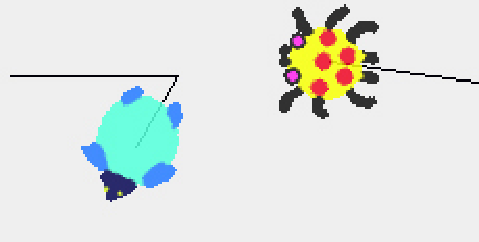
\includegraphics{beasts}
\end{chapterfigure}

The basic look of the robots is rather simple. In this chapter we show you how we can change the shape, the size and the color of robots. We present how you can draw yourselves the appearance of your robots to simulate for example animals.  


\section{Pen Size and Color}
So far the trace left by our robot was black. However, you can change the color of a robot pen sending it the message \ct{penColor: }\index{penColor: aColor} with a color. For example the expression \ct{\caro penColor: Color blue} changes the color of the pen to blue. One of the way to create a color is to send a message with the name of a color to the class \ct{Color} as for example  \ct{Color blue} or \ct{Color yellow}. We will explain colors in the following section. We can also change the size of the robot pen by sending the message \index{penSize:}\ct{penSize:} with a number as argument (\ct{\caro penSize: 5}).  The script~\ref{scr:blueLine} draws a thick blue line while the script~\ref{scr:Stair} draws a strange stair by increasing regularly the pen size.

\begin{scriptwithtitle}{A blue line}\label{scr:blueLine}
| \caro |
\caro := \Turtle new.
\caro \textbf{penColor: Color blue}.
\caro go: 100.
\caro \textbf{penSize: 5}.
\caro go: 100
\end{scriptwithtitle}


\ 


\begin{scriptfig}{turtleMPenSize}{Stair}\label{scr:Stair}
| \caro |
\caro := \Turtle new.
\caro go: 40.
\caro penSize: 2.
\caro go: 40.
\caro penSize: 4.
\caro go: 40.
\caro penSize: 6.
\caro go: 40.
\end{scriptfig}

\ 

Changing the color of the robot itself is also possible using the
method \index{color: aColor}\ct{color:} (\ct{\caro color: Color yellow}). The \scriptref{scr:yellowturtle} asks \ct{daly} to change its color, to go forward while \caro does not move.

\begin{scriptwithtitle}{Two Robots}\label{scr:yellowturtle}
| \caro daly |
\caro := \Turtle new.
daly  := \Turtle new.
daly color: Color yellow.
daly go: 100.
\end{scriptwithtitle}

\section{About Colors}

As previously mentioned, \sq  is an environment built from and using objects. Therefore programming in \sq amounts to creating objects and sending them messages. In particular a \emph{color} is an object created by the class \ct{Color}. To get a color you should send a message to the class \ct{Color}. For example, \ct{Color red} creates the color red. Here is the list of the predefined messages that you can send to create a color to the class \ct{Color}: 
\ct{black}, \ct{veryVeryDarkGray}, \ct{veryDarkGray}, \ct{darkGray}, \ct{gray}, \ct{lightGray}, \ct{veryLightGray}, \ct{veryVeryLightGray}, \ct{white}, \ct{red}, \ct{yellow}, \ct{green}, \ct{cyan}, \ct{blue}, \ct{magenta}, \ct{brown}, \ct{orange}, \ct{lightRed}, \ct{lightYellow}, \ct{lightGreen}, \ct{lightCyan}, \ct{lightBlue}, \ct{lightMagenta}, \ct{lightBrown}, \ct{lightOrange}, \ct{paleBuff}, \ct{paleBlue}, \ct{paleYellow}, \ct{paleGreen} ,\ct{paleRed}, \ct{veryPaleRed}, \ct{paleTan}, \ct{paleMagenta}, \ct{paleOrange}, and \ct{palePeach}.

\Tscrref{scr:colorCreation} shows how to create colors explicitly using the methods \index{r:g:b:}\ct{r: red g: green b: blue} and \index{h:s:v:}\ct{h: hue s: saturation v: brightness}. The arguments of the methods \ct{h:s:v:} and \ct{r:g:b:} should be float numbers ranged from 0 to 1.0. For example the expression \ct{Color r: 1 g:0 b:0} creates the color red equivalent to \ct{Color red}.
Finally the method \index{fromUser}\ct{fromUser} allows you to choose directly a color and show you the color ingredients. For that you need to execute the expression \ct{Color fromUser} using the \menu{print it} menu to get the result of the selection printed.

Print the result by using the print it menu when executing the expression \ct{Color fromUser}).

\begin{scriptfig}{colorFromUser}{Other ways to create colors}\label{scr:colorCreation}
"Produce a pure red"
Color h: 0 s: 1 v: 1
Color r: 1 g:0 b:0

"To choose your color direclty"
Color fromUser
\end{scriptfig}



\section{Changing Robot Shape}
\fprod{this section will change}
Another aspect of a robot that you can change is its shape. Two different shapes a circle and a triangle are proposed by default plus the possibility to draw your own shape as shown later in Section~\ref{sec:drawingTurtle}.

\begin{figure}[h]
\begin{center}
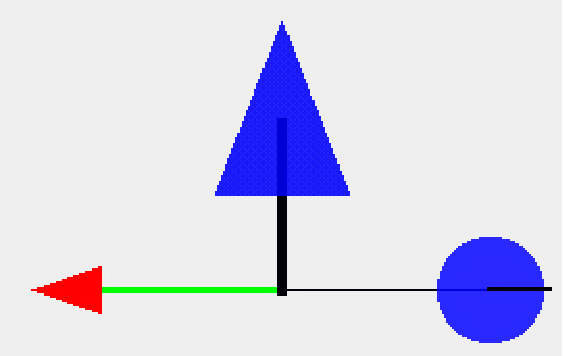
\includegraphics[width=8cm]{shapeAndSize}
\caption{Different robot shapes and size. \label{fig:shapeAndSize}}
\end{center}
\end{figure}

\Tscrref{scr:differentsize} shows how to change the shape of a robot using the message \index{lookLikeTriangle} \ct{lookLikeTriangle} as shown in Figure~\ref{fig:shapeAndSize}. The default shape, the circle, is produced by sending the message   \index{lookLikeCircle} \ct{lookLikeCircle}. 

\begin{scriptwithtitle}{Creating Robots of Different Size and Shape}\label{scr:differentsize}
| \caro daly  big\caro |
\caro := \Turtle new.
\caro \textbf{lookLikeTriangle}.
\caro west.
\caro color: Color red.
\caro penColor: Color green.
\caro penSize: 3.
\caro go: 100.
daly := \Turtle new.
daly \textbf{extent: 60@60}.
daly east.
daly go: 100.
big\caro := \Turtle new.
big\caro \textbf{lookLikeTriangle}.
big\caro \textbf{extent: 100@150}.
big\caro penSize: 5.
big\caro north.
big\caro go: 80.
\end{scriptwithtitle}


\paragraph{Robot Size.}
The second aspect you can change is the size of a robot using the message \index{extent:} \ct{extent: aPoint}, where the values of the point represent the width and height of the rectangle in which the robot is drawn. A point is composed of two numbers separated by the \ct{@} symbol. For example, the point \ct{50@100} represents a rectangle of 50 pixels on 100.







\section{Drawing Your Own Robot}\label{sec:drawingTurtle}
\fprod{this section will change:}
The environment allows you to draw the robot itself and to obtain robots that look like the first figure of this chapter. Now we describe step by step how you can draw your own robot. 

\paragraph{Step1. Getting a Drawing Tool.}
The first step you should perfom is to open the painting tool that is included in \sq. The paint tool is available in the \menu{@@Pica@@} blue flap (Figure~\ref{fig:paintToolCaroFlap}). Therefore drag the small icon of the paint tool in the main screen. This should open the paint tool shown in Figure~\ref{fig:paintOpen}

\begin{figure}
\begin{center}
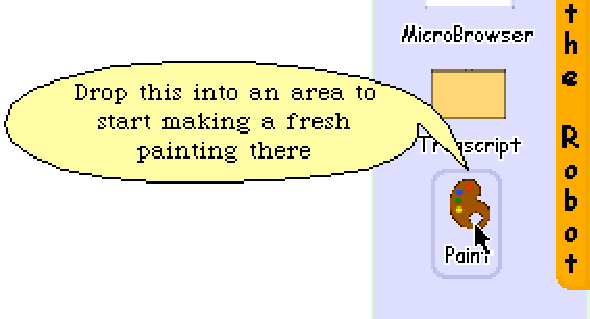
\includegraphics[width=6cm]{paintToolCaroFlap} 
\end{center}
\caption{ \label{fig:paintToolCaroFlap} Getting the painting editor from the blue flap.}
\end{figure}



%\begin{figure}
%\begin{center}
%\includegraphics[width=6cm]{widgetFlaps} \includegraphics[width=6cm]{paint}  
%\end{center}
%\caption{Left: The widget flap. \label{fig:Paint} Right: Getting the painting editor from the widget flap. \label{fig:widgetFlap}}
%\end{figure}

%\begin{figure}
%\begin{center}
%\includegraphics[width=5cm]{gettingPaintEditor}
%\end{center}
%\caption{Getting the painting editor from the object palette. \label{fig:gettingPaintEditor}}
%\end{figure}

\begin{figure}
\begin{center}
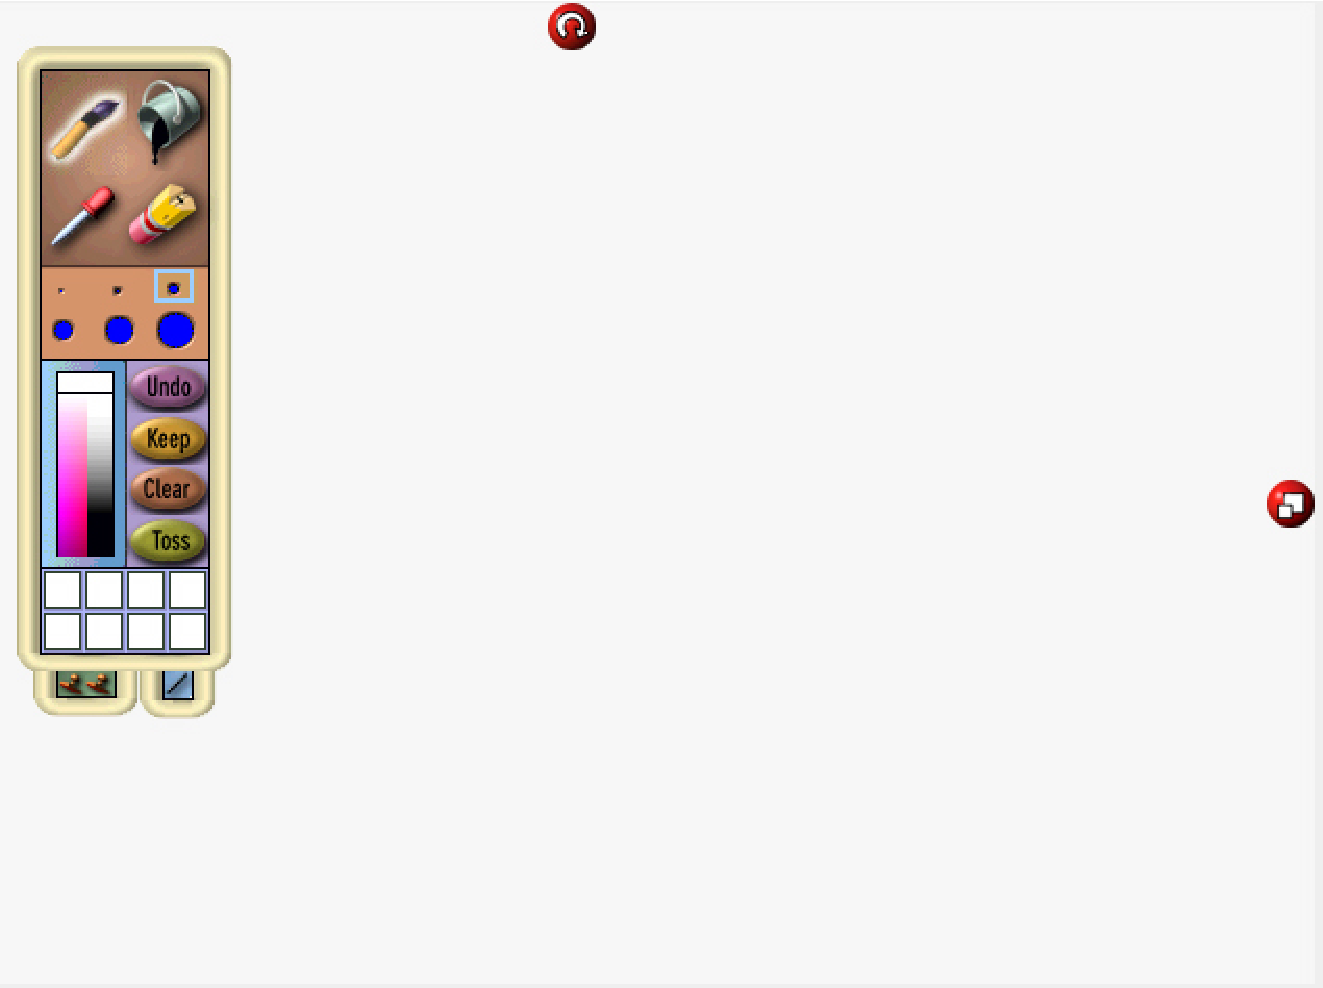
\includegraphics[width=14cm]{paintOpen}
\caption{The painting editor opens. \label{fig:paintOpen}}
\end{center}
\end{figure}

\paragraph{Step2. Drawing  a New Graphics. }
The second step is to draw a new graphics for representing your robot. Draw your robot as if it would point towards the right as shown in Figure~\ref{fig:luth}. The painting editor has the usual facilities such as different brush size, filling region, selecting region as repeated pattern, selecting painting color (see Figure~\ref{fig:palette}). The painting editor has two buttons shown in Figure~\ref{fig:rotate}  to rotate and zoom your drawing. 

\begin{figure}
\begin{center}
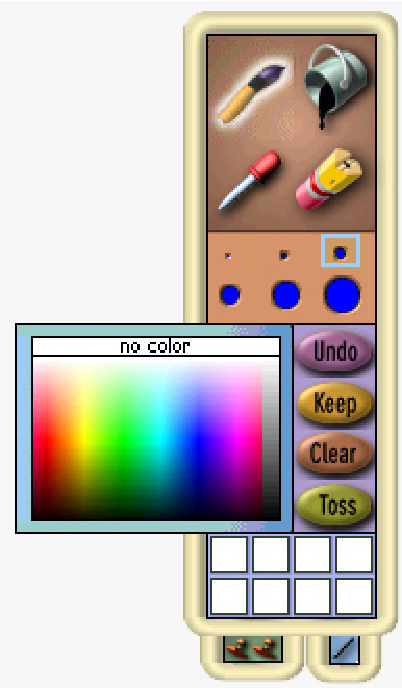
\includegraphics[width=5cm]{palette}
\end{center}
\caption{The painting editor's palette. \label{fig:palette}}
\end{figure}

\begin{figure}
\begin{center}
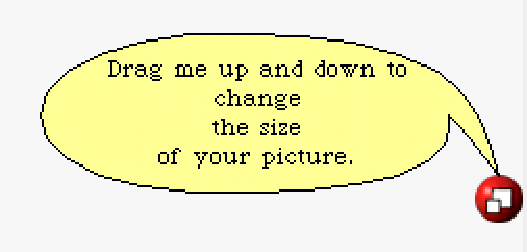
\includegraphics[width=5cm]{zoomButton} 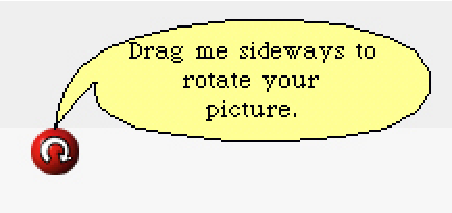
\includegraphics[width=5cm]{rotateButton}
\end{center}
\caption{The zoom and rotate buttons. \label{fig:zoom}\label{fig:rotate}}
\end{figure}


\begin{figure}
\begin{center}
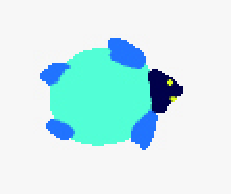
\includegraphics{luth} 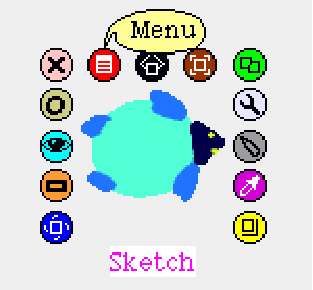
\includegraphics{debugMenu}
\end{center}
\caption{Left: Drawing a new shape pointing toward the east. \label{fig:luth} Right: Getting the red menu. \label{fig:redMenu}}
\end{figure}

\paragraph{Step3. Keeping the Graphics.} Once you are satisfied with your drawing, you should press the button \button{keep}. This closes the editor but leaves your graphics on the screen. Now we have to associate the graphics with the \ct{\Turtle} class. To do so you should activate the halos on the graphics (Option click), click on the red halo as shown in Figure~\ref{fig:redMenu} to pop up a menu, and select the menu item \textbf{keep as robot}. Now you are ready to see if your drawing 
fits well your robot. 

\fprod{this section will change: @@keep as robot@@}
@@keep as robot@@
@@should change the keep to store it into the turtle@@

Execute \tscrref{scr:lookimage} and you should get a new robot with the shape you draw. Note that all the  robots that you will create will be shown using the same graphics. But each of them can still be shown as a triangle or circle.


\begin{scriptwithtitle}{Use of \ct{lookLikeImage}}\label{scr:lookimage}
| \caro luth | 
luth := \Turtle new.
luth  lookLikeImage.
\caro := \Turtle new.
\caro lookLikeCircle.
\end{scriptwithtitle}

\summa

\begin{table}[h]
\centering
\begin{tabular}{||p{3cm}|p{4cm}|p{6.5cm}||} \hline
% after \\ : \hline or \cline{col1-col2} \cline{col3-col4} ...
Method&Description&Example\\[1ex] \hline
\ct{lookLikeCircle}&Change the shape of the receiver to be a circle& \ct{\Turtle new lookLikeCircle}\\ \hline
\ct{lookLikeTriangle}&Change the shape of the receiver to be a triangle&\ct{\Turtle new lookLikeTriangle}\\ \hline
\ct{lookLikeImage}&Change the appareance of the receiver to be as the sketch you paint& \ct{\Turtle new lookLikeImage} \\ \hline

\ct{penColor: aColor}&Change the color of the pen& \ct{\Turtle new penColor: Color blue}\\ \hline
\ct{penSize: aNumber}&Change the size of the pen. The default size is 1.&\ct{\Turtle new penSize: 3}\\ \hline

\ct{color: aColor}&Change the color of the receiver to the specified color& \ct{\Turtle new color: Color yellow}\\ \hline
\ct{extent: aPoint}&Change the size of the receiver. aPoint (w@h) specifies the new size of the receiver as the size of the rectangle. The first number is the width and the second the height. &\ct{\Turtle new extent: 80@100}\\ \hline

\end{tabular}
\end{table}

\ifx\wholebook\relax\else\end{document}\fi



